\section[Resultados y Discusiones]{CAPÍTULO 5:$\ \ \ \ $RESULTADOS Y DISCUSIONES} 
El código desarrollado a lo largo de este trabajo se encuentra disponible en un repositorio público en línea junto con su correspondiente documentación \cite{repo}.

\subsection[Bases de datos de respuestas al impulso]{BASES DE DATOS DE RESPUESTAS AL IMPULSO}

Para tener una medida de la variedad de reverberación presente en los conjuntos de respuestas al impulso reales, generadas y aumentadas, se utilizaron los parámetros $TR_mid$ y $DRR$. En las figuras \ref{fig:cloud_reales}, \ref{fig:cloud_generadas}, y \ref{fig:cloud_aumentadas} se muestran los parámetros acústicos anteriormente mencionados para cada conjunto de respuestas al impulso utilizado.  

\begin{figure}[H]
	\centering{}
	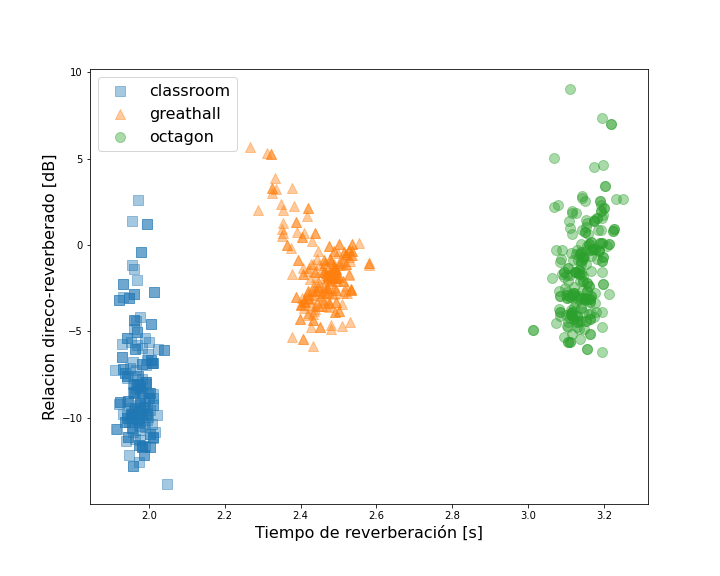
\includegraphics[scale=0.5]{reales.png}
	\caption{Conjunto de respuestas al impulso reales.}
	\label{fig:cloud_reales}
\end{figure}

\begin{figure}[H]
	\centering{}
	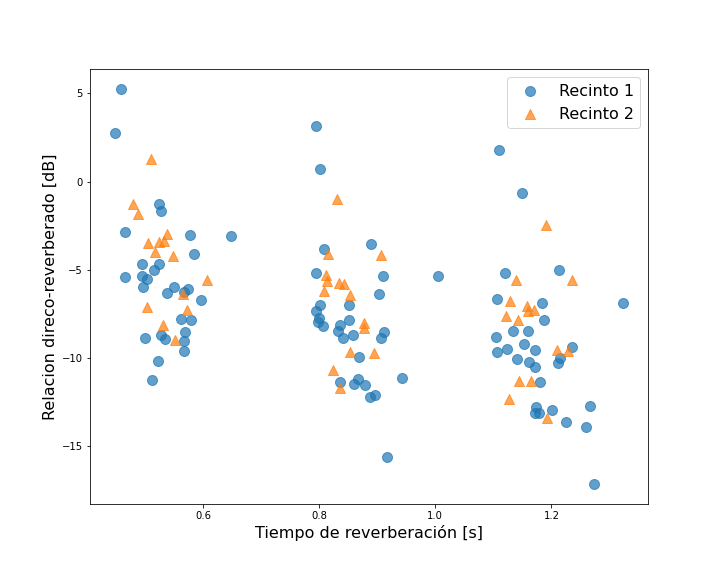
\includegraphics[scale=0.5]{generadas.png}
	\caption{Conjunto de respuestas al impulso generadas.}
	\label{fig:cloud_generadas}
\end{figure}

\begin{figure}[H]
	\centering{}
	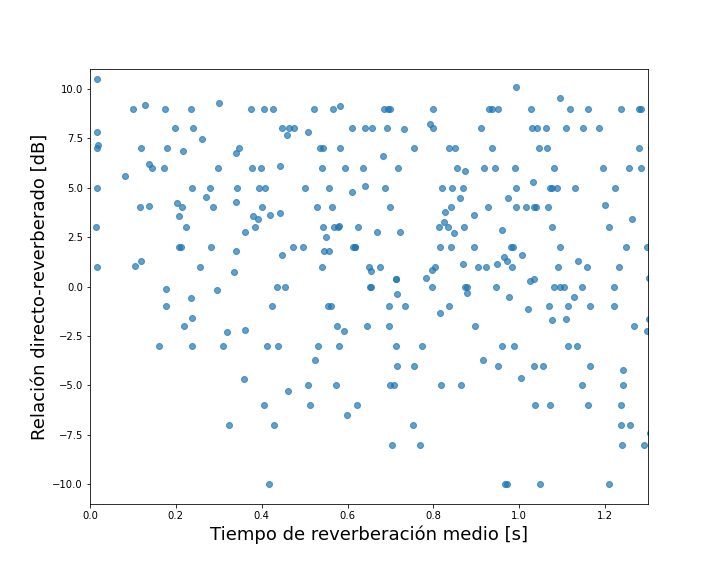
\includegraphics[scale=0.5]{aumentadas.png}
	\caption{Conjunto de respuestas al impulso aumentadas.}
	\label{fig:cloud_aumentadas}
\end{figure}

Del análisis de estos conjuntos utilizando como medida la relación directo reverberado  y el tiempo de reverberación medio se pueden observar algunas particularidades. Respecto a las respuestas al impulso reales, en la figura \ref{fig:cloud_reales} se pueden distinguir tres grandes grupos de puntos de acuerdo a los tres recintos de los cuales fueron obtenidas dichas respuestas. Las variaciones de ambos parámetros acústicos ocurren debido a las diferentes posiciones de micrófono que han sido utilizadas en cada recinto, produciendo variaciones de DRR en un rango de $10 dB$ y de tiempo de reverberación de $2 \ s$ aproximadamente. Pese a estas variaciones, la distribución de los puntos no es uniforme dentro del rango, sin mencionar que no existen respuestas correspondientes a tiempos de reverberación menores a $1.8 \ s$. Algo similar ocurre con las respuestas al impulso generadas que se muestran en la figura \ref{fig:cloud_generadas}. Si bien en este caso se tiene control sobre los puntos centrales de los conjuntos de puntos (se generaron para tiempos de reverberación de $0.5 \ s$, $0.75 \ s$ y $1.0 \ s$) ocurre el mismo fenómeno que con las respuestas al impulso reales, en donde se forman grupos de puntos que no se dispersan uniformemente en el plano. Esto cambia para el tercer conjunto que corresponde a las respuestas al impulso generadas a partir del proceso de aumentación. La dispersión de estas respuestas se observa en la figura \ref{fig:cloud_aumentadas}. A primera vista se observa una mayor uniformidad de los puntos en el plano, ya que no se aprecian conjuntos separados sino más bien una aleatoriedad uniforme a lo largo del rango generado. La uniformidad de la dispersión la podemos atribuir al control que se tiene sobre estos parámetros a la hora de generar las respuestas aumentadas, y la aleatoriedad entre los puntos se debe al hecho de que siempre se parte de una respuesta al impulso real diferente para realizar la aumentación, lo cual produce que el margen entre los parámetros deseados y los obtenidos sea variable. Por otro lado, parece haber una menor cantidad de puntos en la esquina inferior izquierda del grafico, es decir, tiempos de reverberación bajos con relaciones directo-reverberado bajos. Esta es una limitación tanto propia del algoritmo de aumentación como también de la naturaleza de las respuestas al impulso reales, en donde para tiempos de reverberación bajos la energía de la parte tardía de la respuesta es de por sí baja. 


%%%%%%%%%%%%%%%%%%%%%%%%%%%%%%%%%%%%%%%%%%%%%%%%%%%%%%%%%%%%%%%%%%%%%


\subsection[Funcionamiento del sistema]{FUNCIONAMIENTO DEL SISTEMA}
En la figura \ref{fig:mean and std of nets} se muestra una instancia de ejemplo del funcionamiento del algoritmo de dereverberación implementado. Durante el entrenamiento, el espectrograma reverberado ingresa a la red neuronal para procesarse y generar una máscara de amplitud. En la salida, esta máscara se aplica sobre el mismo espectrograma reverberado de entrada para generar el espectrograma dereverberado. Esta es la salida de la red, la cual se compara contra el espectrograma anecoico dentro de la función de costo para poder propagar el error a lo largo de los pesos sinápticos de la red neuronal. Luego, a la hora de hacer predicciones, solo se necesita ingresar un espectrograma reverberado para que la red estime una máscara de amplitud con la cual pueda generarse el espectrograma dereverberado. Cabe aclarar que a lo largo de estos procesos se trabaja únicamente sobre la magnitud de la STFT, a lo que se hace referencia como espectrograma.  
\begin{figure}[H]
        \centering
        \begin{subfigure}[b]{0.475\textwidth}
            \centering
            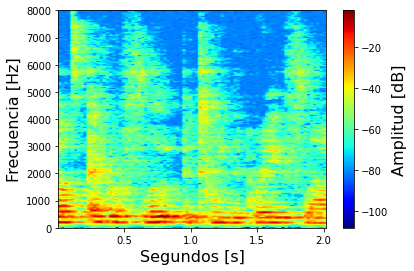
\includegraphics[width=\textwidth]{espectro_in.png}
            \caption[Network2]%
            {{\small Espectrograma reverberado}}    
            \label{fig:mean and std of net14}
        \end{subfigure}
        \hfill
        \begin{subfigure}[b]{0.475\textwidth}  
            \centering 
            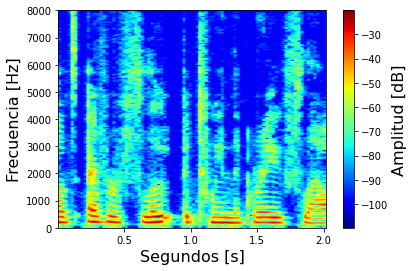
\includegraphics[width=\textwidth]{espectro_target.png}
            \caption[]%
            {{\small Espectrograma anecoico}}    
            \label{fig:mean and std of net24}
        \end{subfigure}
        \vskip\baselineskip
        \begin{subfigure}[b]{0.475\textwidth}   
            \centering 
            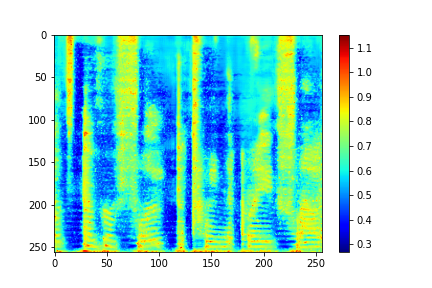
\includegraphics[width=\textwidth]{mascara.png}
            \caption[]%
            {{\small Mascara estimada por la red}}    
            \label{fig:mean and std of net34}
        \end{subfigure}
        \hfill
        \begin{subfigure}[b]{0.475\textwidth}   
            \centering 
            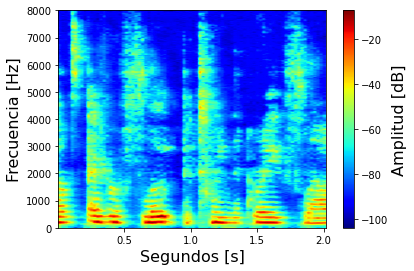
\includegraphics[width=\textwidth]{espectro_out.png}
            \caption[]%
            {{\small Espectrograma dereverberado}}    
            \label{fig:mean and std of net44}
        \end{subfigure}
        \caption[ The average and standard deviation of critical parameters ]
        {\small Ejemplo de procesamiento de audio reverberado} 
        \label{fig:mean and std of nets}
    \end{figure}
    
Se puede observar que el aprendizaje de la red neuronal desemboca en la generación de máscaras de amplitud que mantienen la ganancia de las componentes propias del habla anecoica y atenúan las componentes introducidas por el fenómeno de la reverberación. La atenuación de las componentes reverberantes ocurre con mayor precisión para frecuencias bajas, en donde hay más energía. A pesar de esto, se pueden observar rasgos del espectro reverberado aun presentes en el espectro dereverberado, lo que es de esperarse debido a que el proceso únicamente esta aplicando un filtro de amplitud por sobre la magnitud del espectro reverberado.

%% CONSIDERAR AGREGAR EJEMPLOS DE MASCARAS BUENAS Y MALAS
%%%%%%%%%%%%%%%%%%%%%%%%%%%%%%%%%%%%%%%%%%%%%%%%%%%%%%%%%%%%%%%%%%%%%%%%%%


\subsection[Reconstrucción de audio dereverberado]{RECONSTRUCCIÓN DE AUDIO DEREVERBERADO}
El proceso de dereverberación de los audios sucede sobre la magnitud de los espectros STFT de los audios con reverberación. Una vez estimada la magnitud del espectro dereverberado, es necesario combinar esta magnitud con información de fase, para poder conformar un espectrograma complejo apto para antitranformarse y pasar del dominio temporal-frecuencial al dominio temporal (información de audio). Un ejemplo de los espectros de magnitud y fase para un audio con reverberación y sin reverberación se muestra en la figura \ref{fig:fases}.

\begin{figure}[H]
\centering
\begin{subfigure}{.5\textwidth}
  \centering
  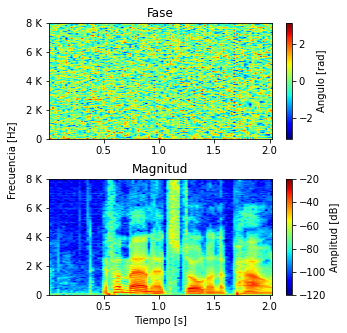
\includegraphics[scale=0.65]{fase_clean.png}
  \caption{Audio sin reverberación}
  \label{fig:fase_sub1}
\end{subfigure}%
\begin{subfigure}{.5\textwidth}
  \centering
  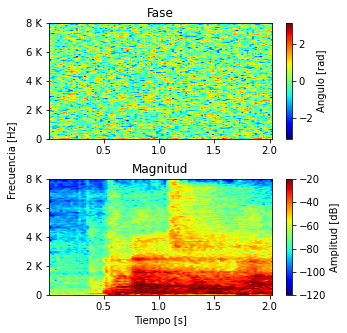
\includegraphics[scale=0.65]{fase_reverb.png}
  \caption{Audio con reverberación}
  \label{fig:fase_sub2}
\end{subfigure}Sin embargo
\caption{Espectrogramas de magnitud y fase de los audios para entrenamiento}
\label{fig:fases}
\end{figure} 

Se puede apreciar que los espectros de fase parecen contener poca información estructural a comparación de los espectros de magnitud. Tanto la fase del audio con reverberación como la fase del audio sin reverberación parecen contener información aleatoria, y a simple vista son similares entre sí. Es por esto que el proceso de dereverberación se realiza solo sobre la magnitud de la STFT. 

Para determinar la fase del nuevo espectro de magnitud estimado por la red (dereverberado), se consideraron dos alternativas: utilizar directamente la fase del espectro con reverberación o bien utilizar el método iterativo de Griffin-Lim para estimar la fase a partir de la magnitud dereverberada. Este último método iterativo puede inicializarse con una fase determinada (como la fase del audio reverberado) para aprovechar información existente de manera de mejorar la estimación o puede inicializarse de manera aleatoria. 
Para determinar el número necesario de iteraciones a utilizar en el algoritmo de Griffin-Lim se evaluó la evolución de las métricas utilizadas en este trabajo (SDR, SRMR y ESTOI) en relación al número de iteraciones en la obtención de la fase. En la figura \ref{fig:iteraciones} se pueden observar estas relaciones para cada métrica, teniendo en cuenta que se utilizó el algoritmo inicializado desde una fase aleatoria. Se puede apreciar que los valores se estabilizan al aproximarse a 100 iteraciones, siendo este el número de iteraciones que se utilizó para las pruebas subsiguientes.     

\begin{figure}[H]
	\centering{}
	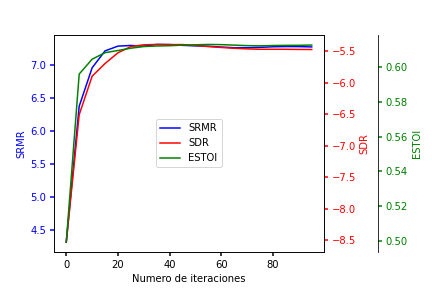
\includegraphics[scale=0.9]{iteraciones.png}
	\caption{Influencia del número de iteraciones del algoritmo de Griffin-Lim.}
	\label{fig:iteraciones}
\end{figure}

En la tabla \ref{table:fases} se muestra el resultado de la comparación entre las distintas alternativas para la determinación de la fase del espectro dereverberado. Para hacer esta comparación se utilizó audio reverberado como referencia, sobre el cual se calculan las métricas objetivas SDR, SRMR y ESTOI. Luego, se implementó cada alternativa de obtención de fase para el espectro de magnitud dereverberado con el fin de generar información de audio y calcular estas mismas métricas. En la tabla se expresan las variaciones de las métricas para cada alternativa con respecto al audio reverberado. Se puede observar que la principal diferencia ocurre sobre el parámetro SDR. La reconstrucción de fase utilizando el algoritmo de Griffin-Lim inicializado de manera aleatoria empeora el resultado de esta métrica, lo cual es un efecto contrario al deseado. Sin embargo, utilizando este algoritmo inicializado con la fase reverberada genera una mejora. Finalmente, la dereverberación utilizando directamente la fase reverberada produce una mejora mucho mayor que los metodos iterativos previamente mencionados. Para las otras dos métricas, SRMR y ESTOI, los métodos iterativos producen mejores resultados que la utilización directa de la fase reverberada, pero las diferencias entre las alternativas son menores.

\begin{table}[H]
\centering
\caption{Comparación de métodos de reconstrucción de espéctrograma complejo para generar audio}
\begin{tabular}{|l|l|l|l|}
\hline
                                                                               & \textbf{SDR}                         & \textbf{SRMR}                      & \textbf{ESTOI} \\ \hline
\textit{Audio reverberado (referencia)}                                        & \multicolumn{1}{c|}{\textit{- 3.11}} & \multicolumn{1}{c|}{\textit{1.73}} & \textit{0.29}  \\ \hline
\Delta $\ $ Dereverberación con fase reverberada                      & +4.27                                & +4.53                              & +0.31          \\
\Delta $\ $ Dereverberación Griffin-Lim iniciado con fase reverberada & +1.38                                & +5.13                              & +0.33          \\
\Delta $\ $ Dereverberación Griffin-Lim iniciado con fase aleatoria   & -2.92                                & +5.24                              & +0.33          \\ \hline
\end{tabular}
\label{table:fases}
\end{table}

De los resultados obtenidos sobre las distintas alternativas estudiadas para obtener el espectro de fase que complemente a la magnitud dereverberada generada se puede remarcar en primer lugar que las métricas utilizadas no siempre reflejan con fidelidad lo que ocurre en la percepción auditiva de los resultados. Durante la realización de estas pruebas, ocurrió que el método que arrojaba mejores resultados sobre las métricas no era el que mejor se percibia auditivamente. También, ocurrió que sobre determinados ejemplos ambas alternativas generaban distorsiones subjetivamente similares pero producían resultados notoriamente distantes sobre las métricas. De igual manera, la utilización de la fase reverberada de manera directa resultó ser el método más robusto frente a las métricas. Esto, sumado a su utilización en otros trabajos del estado del arte AGREGAR REFERENCIA hizo que esta alternativa sea la escogida a lo largo de este trabajo. Sin embargo, este análisis de fase deja en evidencia la falta de correlación de ciertas métricas como el SDR con la percepción auditiva de los resultados. Por cuestiones como esta existen nuevas variantes de estas métricas que buscan generar una mayor robustez frente a estas cuestiones de reconstrucción de audio \cite{sdr_fail}. 
%%%%%%%%%%%%%%%%%%%%%%%%%%%%%%%%%%%%%%%%%%%%%%%%%%%%%%%%%%%%%%%%%%%%%%%%%%%%%%%%%%%%%

\subsection[Dereverberación del habla y manejo de datos]{DEREVERBERACIÓN DEL HABLA Y MANEJO DE DATOS}

Para las evaluaciones se tuvieron en cuenta tres conjuntos de datos de acuerdo al tipo de respuestas al impulso utilizadas para generar la reverberación: reales, generadas y aumentadas. Para medir el desempeño de la tarea de dereverberación, las métricas se evaluan sobre los conjuntos reverberados y luego sobre sus correspondientes resultados dereverberados. Los resultados de estas métricas para los conjuntos reverberados se puede observar en la tabla \ref{table:resultados_reverb}. 

\begin{table}[H]
\centering
\caption{Resultados de las métricas sobre los conjuntos reverberados}
\begin{tabular}{|c|c|c|c|}
\hline
Conjunto   & \textbf{SDR} & \textbf{SRMR} & \textbf{ESTOI} \\ \hline
Reales     & -3.94        & 1.22          & 0.28           \\
Generadas  & 2.89        & 2.53          & 0.46           \\
Aumentadas & 8.09        & 3.19          & 0.64           \\ \hline
\end{tabular}
\label{table:resultados_reverb}
\end{table}


Los resultados obtenidos para el primer conjunto de pruebas definidos en la tabla \ref{tab:pruebas} se expresan en las figuras \ref{fig:1_SDR}, \ref{fig:1_SRMR} y \ref{fig:1_ESTOI} para las variaciones de las métricas SDR, SRMR y ESTOI respectivamente. 

\begin{figure}[H]
	\centering{}
	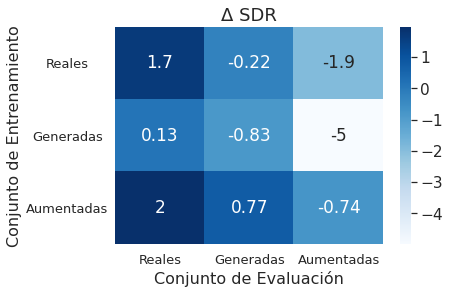
\includegraphics[scale=0.65]{prueba1_SDR.png}
	\caption{Variaciones de SDR para el primer conjunto de pruebas.}
	\label{fig:1_SDR}
\end{figure}

\begin{figure}[H]
	\centering{}
	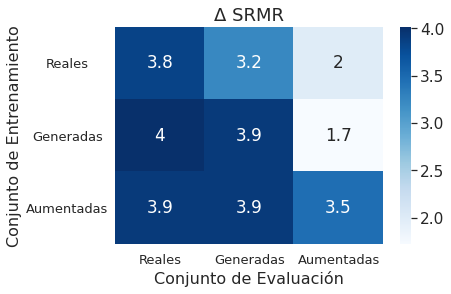
\includegraphics[scale=0.65]{prueba1_SRMR.png}
	\caption{Variaciones de SRMR para el primer conjunto de pruebas.}
	\label{fig:1_SRMR}
\end{figure}

\begin{figure}[H]
	\centering{}
	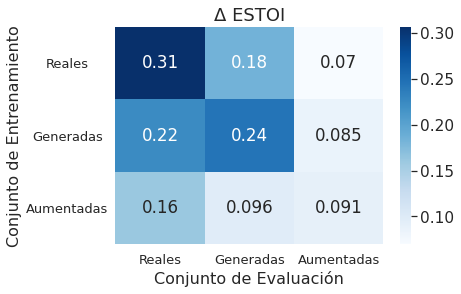
\includegraphics[scale=0.65]{prueba1_ESTOI.png}
	\caption{Variaciones de ESTOI para el primer conjunto de pruebas.}
	\label{fig:1_ESTOI}
\end{figure}

Del primer conjunto de pruebas se esperaba obtener los mejores resultados para aquellos casos en los que el conjunto de entrenamiento y el conjunto de evaluación coinciden. Esto ocurrió para la evaluación con la métrica ESTOI. Para las otras métricas, el comportamiento esperado ocurrió en general para los conjuntos formados con respuestas al impulso reales y aumentadas, pero no para las generadas. Particularmente, utilizar respuestas al impulso aumentadas durante el entrenamiento produjo mejores resultados al evaluar sobre respuestas al impulso generadas que usando respuestas al impulso generadas durante el entrenamiento. Esto puede deberse al hecho de que, si bien ambos conjuntos contienen tiempos de reverberación del mismo rango, las respuestas al impulso aumentadas tienen una distribución más uniforme a lo largo de este rango.

Los resultados correspondientes al segundo conjunto de pruebas definido en la tabla \ref{tab:pruebas_combinadas} se muestran en las figuras \ref{fig:2_SDR}, \ref{fig:2_SRMR} y \ref{fig:2_ESTOI} para las variaciones de las métricas SDR, SRMR y ESTOI respectivamente.

\begin{figure}[H]
	\centering{}
	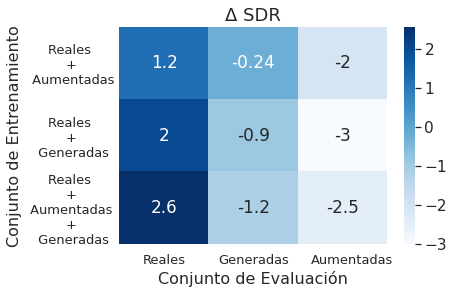
\includegraphics[scale=0.65]{prueba2_SDR.png}
	\caption{Variaciones de SDR para el segundo conjunto de pruebas.}
	\label{fig:2_SDR}
\end{figure}

\begin{figure}[H]
	\centering{}
	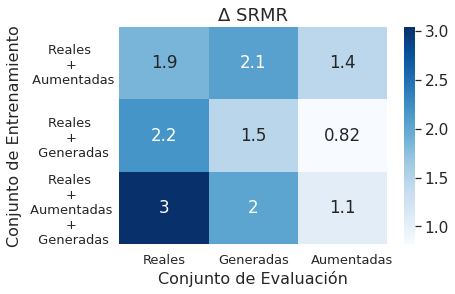
\includegraphics[scale=0.65]{prueba2_SRMR.png}
	\caption{Variaciones de SRMR para el segundo conjunto de pruebas.}
	\label{fig:2_SRMR}
\end{figure}

\begin{figure}[H]
	\centering{}
	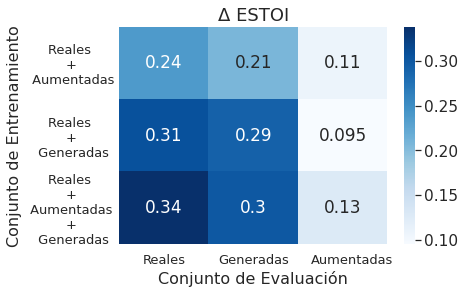
\includegraphics[scale=0.65]{prueba2_ESTOI.png}
	\caption{Variaciones de ESTOI para el segundo conjunto de pruebas.}
	\label{fig:2_ESTOI}
\end{figure}

Para el segundo conjunto de pruebas se combinaron tipos de respuestas al impulso en la conformación de los datos de entrenamiento y se volvió a evaluar en los mismos conjuntos de la primera prueba, asegurándose que el número de instancias de entrenamiento se mantenga fijo en todas las pruebas. Se debe tener en consideración que es de mayor importancia para éste trabajo evaluar el rendimiento al evaluar sobre respuestas al impulso reales, ya que es el objetivo principal del sistema implementado. En esta prueba, para todas las métricas los mejores resultados se obtuvieron al combinar los tres tipos de datos en la conformación del conjunto de entrenamiento. Es decir, una mayor diversidad de impulsos presentes a la hora de generar los datos de entrenamiento desemboca en una mejora en el rendimiento del sistema. Además, la combinación de respuestas al impulso reales-generadas arrojó mejores resultados que la combinación reales-aumentadas para todas las métricas. Esto puede deberse al hecho de que las respuestas al impulso aumentadas si bien varían la pendiente de caída de la cola reverberante, mantienen el mismo perfil frecuencial que las respuestas al impulso reales de las que provienen. En este aspecto, las respuestas al impulso generadas pueden enriquecer en mayor medida la diversidad de los datos utilizados aportando nuevos perfiles de tiempo de reverberación, lo cual puede llevar a mejores resultados generales. 
%%%%%%%%%%%%%%%%%%%%%%%%%%%%%%%%%%%%%%%%%%%%%%%%%%%%%%%%%%%%%%%%%%%%%%%%%%%%%%%%%%%5


\subsection[Aprendizaje por curriculum]{APRENDIZAJE POR CURRICULUM}
Para evaluar la influencia del ordenamiento de los datos en el proceso de entrenamiento en primer lugar se generó una base de datos de respuestas al impulso asegurando una adecuada dispersión de los parámetros acústicos de relación directo-reverberado y tiempo de reverberación medio. Para poder conseguir esto, se partió de la base de datos de respuestas al impulso reales C4DM y se aplicó el método de aumentación. Esta vez se generaron tiempos de reverberación medio desde $0.1 \ s$ a $3.5 \ s$ y relaciones directo-reverberado de $-10 \ dB$ a $10 \ dB$. En la figura \ref{fig:cl_impulsos} se puede observar la dispersión de los parámetros acústicos mencionados en el conjunto de respuestas al impulso conformado.

\begin{figure}[H]
	\centering{}
	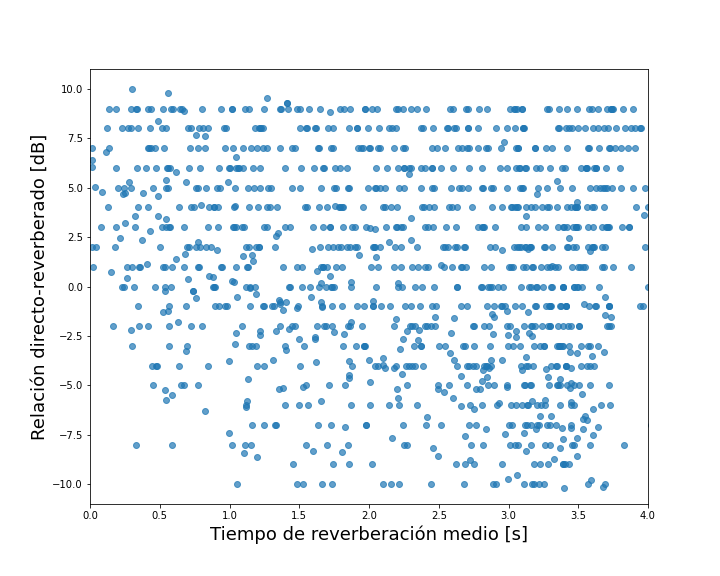
\includegraphics[scale=0.60]{cl_impulsos.png}
	\caption{Respuestas al impulso generadas por aumentación.}
	\label{fig:cl_impulsos}
\end{figure}

Partiendo de la información del tiempo de reverberación medio de cada respuesta al impulso, se generaron pares de audios anecoicos-reverberados junto con un registro que indicaba que tiempo de reverberación medio correspondía con cada audio reverberado. Este registro se utilizó para conformar los esquemas de entrenamiento que fueron evaluados. Entonces, se organizaron los datos de entrenamiento de tres maneras: con tiempos de reverberación creciences, decrecientes y aleatorios. Cabe aclarar que la red se entrenó por una sola época sobre estos conjuntos de datos. Una vez realizado el entrenamiento, se utilizó el modelo entrenado para hacer predicciones sobre audios reververados y se calcularon las métricas objetivas sobre los resultados de cada variante. En las figuras \ref{fig:cl_sdr}, \ref{fig:cl_srmr}, y \ref{fig:cl_estoi} se muestran los resultados obtenidos para las métricas SDR, SRMR y ESTOI respectivamente. 

\begin{figure}[H]
	\centering{}
	\includegraphics[scale=0.75]{cl_SDR.png}
	\caption{Comparación de SDR entre tipos de ordenamiento de datos durante el entrenamiento.}
	\label{fig:cl_sdr}
\end{figure}

\begin{figure}[H]
	\centering{}
	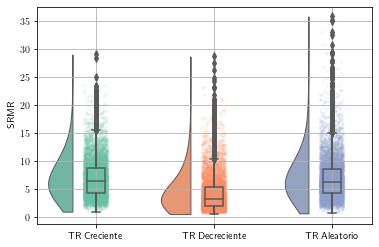
\includegraphics[scale=0.75]{cl_SRMR.png}
	\caption{Comparación de SRMR entre tipos de ordenamiento de datos durante el entrenamiento.}
	\label{fig:cl_srmr}
\end{figure}

\begin{figure}[H]
	\centering{}
	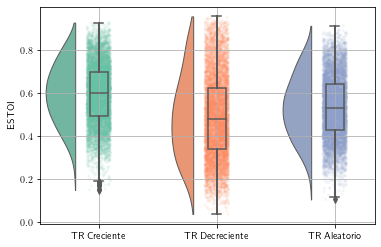
\includegraphics[scale=0.75]{cl_ESTOI.png}
	\caption{Comparación de ESTOI entre tipos de ordenamiento de datos durante el entrenamiento.}
	\label{fig:cl_estoi}
\end{figure}

A primera vista se puede percibir que para todas las métricas el resultado obtenido para el entrenamiento con tiempos de reverberación crecientes es el mejor, el resultado obtenido para el entrenamiento con tiempos de reverberacón decrecientes es el peor, y el resultado para el entrenamiento con tiempos de reverberación aleatorios esta en un punto medio entre los dos anteriores, en ocasiones más cerca del mejor y en ocasiones más cerca del peor. Para ilustrar mejor este comportamiento, en la tabla \ref{table:resultados_reverb} se muestran las medianas de las métricas obtenidas para cada esquema de entrenamiento. 

\begin{table}[H]
\centering
\caption{Medianas correspondientes a cada esquema de entrenamiento.}
\begin{tabular}{|c|c|c|c|}
\hline
               & \textbf{$\tilde{X}_{SDR}$} & \textbf{$\tilde{X}_{SRMR}$} & \textbf{$\tilde{X}_{ESTOI}$} \\ \hline
TR Creciente   & 3.54         & 6.37          & 0.59           \\ \hline
TR Decreciente & 1.24         & 3.25          & 0.47           \\ \hline
TR Aleatorio   & 1.61         & 6.24          & 0.53           \\ \hline
\end{tabular}
\label{table:resultados_reverb}
\end{table}

Finalmente, con estos resultados se pudo corroborar el impacto del ordenamiento de los datos de entrenamiento en el rendimiento final del sistema. En este caso, la complejidad de los datos se asoció al tiempo de reverberación de cada instancia. Con esto, al entrenar con datos ordenados por tiempo de reverberación de manera creciente, es decir, iniciando con tiempos de reverberación bajos y aumentando progresivamente el tiempo de reverberación se obtuvieron mejores resultados para todas las métricas. También se comprobó que el ordenamiento inverso produce el peor resultado de los tres, y el orden aleatorio cae en un punto medio entre estos dos casos. Esto es consistente con la teoría de la técnica de aprendizaje por curriculum. En primera instancia, para tiempos de reverberación bajos, es sencillo para la red neuronal mantener el sonido directo que es predominante en la señal debido a la escasa reverberación (la máscara ideal se asemeja a una máscara unitaria). Esta información aprendida un primer momento guía en cierta medida al algoritmo para ir aprendiendo de instancias progresivamente más complejas en donde la energía proveniente de la reverberación es cada vez mayor. 
